\chapter{Introduction}
\label{chapter:Introduction}

The Internet today is a vast source of information curated by real people. In recent times, the popularity of websites like Twitter, Reddit, and Wordpress has shown that every day, more and more people are getting comfortable with expressing their inner feelings on the web, irrespective of whether they feel good or bad. Negative feelings expressed this way provide an important indicator of what might be going wrong in their lives, or what may ultimately lead up to something more tragic or even terminal. In some cases, factors leading to suicide can be identified early on by looking at the physical and verbal behavior of the person under consideration. Public availability of a larger set of data that may contain content posted by emotionally distressed people, and non-availability of a system that can analyze such data to find such people is a clear problem. This thesis attempts to address this problem by applying machine learning techniques to build such a system that is able to find instances of emotionally distressed content on the Internet. This can then serve as a first step towards providing further help to such people, possibly in the form of human intervention.

\section{Machine learning and text classification}
Machine learning is a branch of computer science that deals with building and analyzing systems that are able to learn from data. Algorithms based on such analysis involve constructing a model from a given dataset, and then using this model to perform required tasks. Machine learning techniques can broadly be divided into two categories - supervised learning, and unsupervised learning.

\begin{itemize}
    \item{
    Supervised Learning\\
    Methods falling in this category operate in two phases. In the first step, the availability of training data is assumed, which is used to build a model so that it takes into account the structure of the given dataset. In the second step, this model is used to make predictions on the testing data (the real world data). This is the data that the model has not seen yet, and is required to make predictions on.
    }
    \item{
    Unsupervised Learning\\
    Methods falling under this category operate in a single phase. It starts with a model with zero knowledge about the structure of the given dataset. As data is fed into the model, it continuously learns the structure of the given dataset and calculates the predictions based on this knowledge. The main difference between this family of algorithms and supervised learning algorithms is the presence/absence of training labels.
    }
\end{itemize}

The primary focus in this thesis remains on supervised learning methods.\\

Text classification is a subset of machine learning algorithms used to assign specific categories to pieces of data. More precisely, given some sample information (such as what kind of data points are to be assigned to which category), these algorithms allow for assigning categories to data points in the future. Under the scope of this thesis, the data is always assumed to be English-text. Since machine learning algorithms only deal with real numbers, a necessary first step is the conversion of natural language text into real numbers. The work presented in this thesis makes extensive use of supervised text classification algorithms.

\section{Problem Definition}
A large portion of the nearly one million people who die every year from suicide includes young people. In recent times, these people have started to express their inner feelings on the web, on websites like Twitter, Wordpress, Reddit, and many others. Reddit \cite{reddit} is one of the very popular websites that people use to express their emotions. Figure~\ref{fig:reddit_happy} shows one such section of Reddit that people use to express positive feelings, while Figure~\ref{fig:reddit_suicidewatch} shows some of the stories that were posted by people (on another section of Reddit) experiencing feelings like depression and loneliness. Suicide is a medical condition that has the potential to be detected early on, by observing the physical and verbal behavior of the person under concern. The work presented in this thesis exploits these two facts, and attempts to build a system that can monitor the public feed of Internet websites such as Twitter (on which people post about what they feel) and detect the content that may have been posted by a person under emotional distress.\\

\begin{figure}
    \centering
    
\includegraphics[width=\textwidth,scale=0.5]{reddit_happy.png}
    \caption{\href{http://www.reddit.com/r/happy}{``/r/happy''}, the section of the website Reddit where people post content when they are happy and want to share it with everyone else}
    \label{fig:reddit_happy}
\end{figure}

\begin{figure}
    \centering
    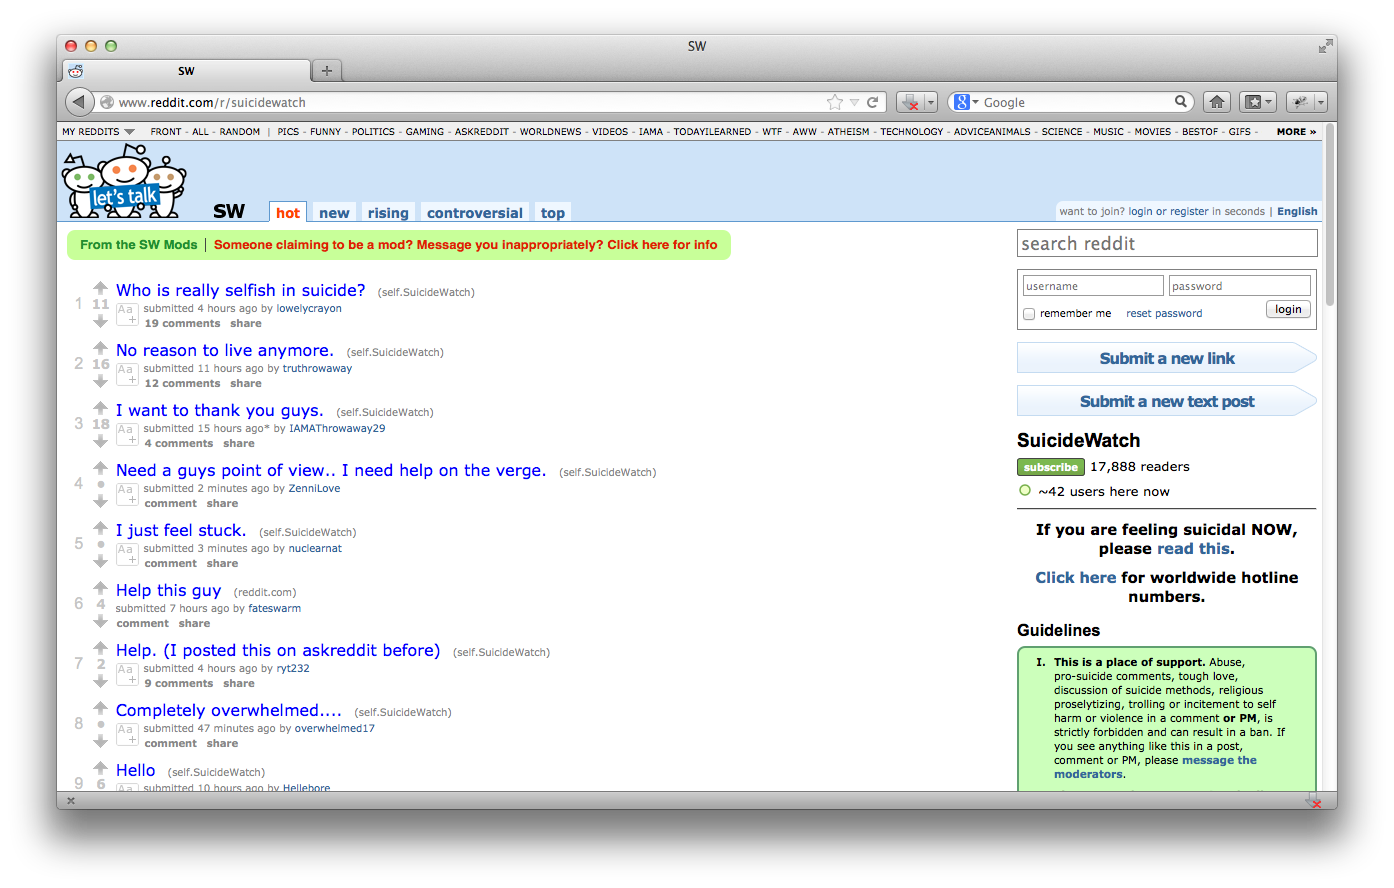
\includegraphics[width=\textwidth,scale=0.5]{reddit_suicidewatch.png}
    \caption{\href{http://www.reddit.com/r/suicidewatch}{``/r/suicidewatch''}, the section of Reddit where people post when they are depressed, or are on the verge of taking their own lives}
    \label{fig:reddit_suicidewatch}
\end{figure}

Pointing out the exact phrases which lead one to believe that a person may be under some degree of emotional distress is a problem best handled by psychologists and linguists. Even though prediction with machine learning algorithms is less sophisticated than human classification, it is known (and also presented in this thesis) that such techniques can identify and categorize the sentiment of a piece of text to a reasonable accuracy. A person may be under emotional distress if he/she posts content which is indicative of sentiments and/or actions like depression, suicide, loneliness, and helplessness. During the work performed in this thesis, the following categories of phrases were found indicative of whether or not a person needs help.\\

\begin{itemize}
    \item{
    Direct\\
    Phrases such as \emph{``thoughts of suicide make me happy''}, \emph{``I have a rope around my neck''} or \emph{``my suicide note''} indicate in a very straightforward manner that the author is not only depressed, but is also on the path of taking his/her own life. Such phrases are very direct indicators of the emotional condition of the person.
    }
    \item{
    Indirect\\
    Phrases such as \emph{``I don't know anything anymore''} or \emph{``Need someone to talk to''} or \emph{``Please help''} indicate that the person who is posting such content does not necessarily want to kill themselves yet, but they are not in a very good emotional health either. Such words indicate that this person is under depression, or is feeling lonely. Even though they may not be suicidal yet, such a dramatic and tragic event might be the next step in their lives.
    }
\end{itemize}

Both the category of phrases indicate that the emotional health of the person under consideration is not normal, and may need attention.\\

The work presented in this thesis tackles this problem by following a two-step approach. In the first step, various text classification algorithms are explored and evaluated that could be a good fit for the problem at hand (identification of text which may or may not have been posted by a depressed person). In the second step, these algorithms are used to build a system that proactively looks for content on the Internet (on places like Twitter), and identifies people who have been posting emotionally distressed content. The system also allows for making improvements to its abilities by tapping into crowd intelligence, which distinguishes the problem being addressed from normal text classification problems. A detailed explanation of this can be found in Chapter~\ref{chapter:Experiments}. This system then serves as a first step towards extending a helpful hand to people who need it.
